%Purpose:
%This is a beamer slide show presentation template.
%
%Author:
%Larz White, University of Idaho, Physics Department: Nuclear Theory Group
%
\documentclass[10pt,serif]{beamer}
%============================packages and commands I use: remove/add them as necessary=============
\usepackage{graphicx,mathtools,amssymb,multirow,braket,slashed,bbm}
\newcommand{\bvec}[1]{\boldsymbol{#1}}
\newcommand{\rb}[1]{\left(#1\right)}
\newcommand{\abs}[1]{\left|#1\right|}
%================Presentation Layout: Make necessary changes=======================================
%
%Change slide theme and appearance
	\usetheme{Malmoe}
	\usecolortheme{crane}
	\useoutertheme{shadow}
	\useinnertheme{rounded}
	\beamertemplatenavigationsymbolsempty
%
%Footnote setup
%	define a symbol footnote for slide references
%	use: \symbolfootnote[num]{text}
%	num=1 --> *   num=2 --> dagger   num=3 --> double dagger   num=4 --> ?
	\long\def\symbolfootnote[#1]#2{\begingroup
	\def\thefootnote{\fnsymbol{footnote}}\footnote[#1]{\tiny #2}\endgroup}
%==================================================================================
\title[Microscopic nuclear effective interactions\hspace{2em}\insertframenumber/
\inserttotalframenumber]{Development and applications of microscopic nuclear effective interactions}
\author{Larz White}
\institute{University of Idaho, Department of Physics}
\date{May 2, 2012}
\logo{\vspace{-1.5em}
\includegraphics[width=1.8cm]{ui_logo}}
\begin{document}
\begin{frame}
\titlepage
\scriptsize{Advisor: Dr. Francesca Sammarruca\\PhD Preliminary Exam Part $\mathrm{I{\hspace{-0.02cm}}I}$}
\end{frame} 
\section{Introduction}
\begin{frame}
\frametitle{Brief overview of nuclear physics: A short video}
\end{frame}
\subsection{Overview}
\begin{frame}
\frametitle{Overview}
\begin{itemize}
\item Introductory comments.
\item \structure{Overview of the field and predictions}
\begin{enumerate}
\item Our starting point is a realistic nucleon-nucleon potential developed within a relativistic scattering equation.
\item Use this as input to calculate the properties of a system known as nuclear matter, in particular its equation of state (EoS).
\item Use the EoS as input to predict observables.
\end{enumerate}
\item Recent work and long range thesis plans.
\end{itemize}
\end{frame}
\subsection{Motivation}
\begin{frame}
\frametitle{Motivation}
\begin{itemize}
\item Improving our understanding of nuclear matter, particularly in the presence of different
neutron and proton concentrations, is one of the goals stated by the Nuclear Science Advisory Committee.
\begin{center}
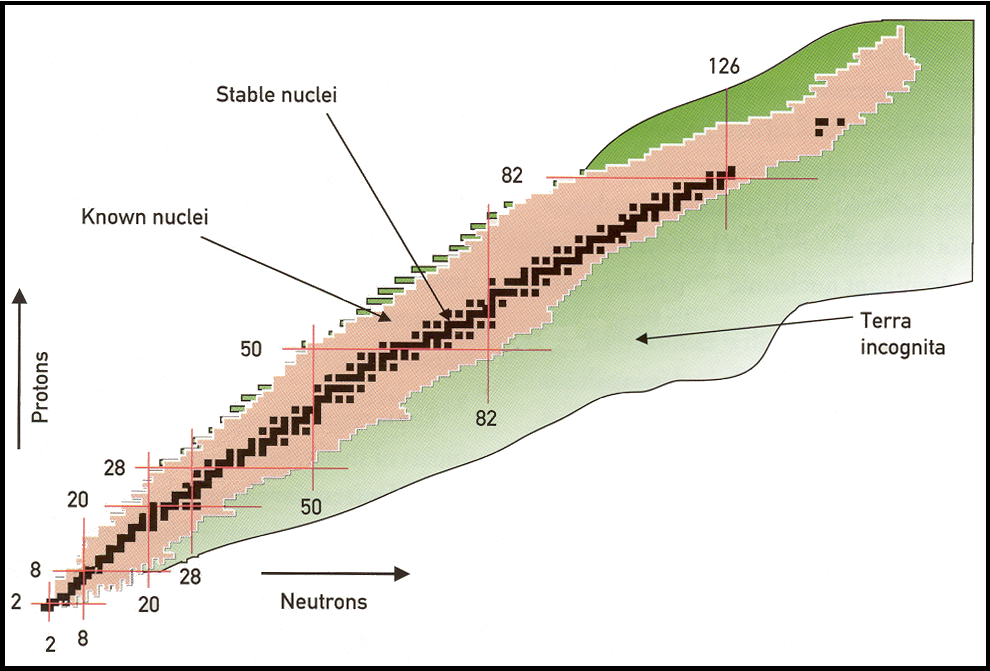
\includegraphics[width=5.2cm,height=4cm]{nuclearlandscape.jpg}
\end{center}
\item Much of the nuclear landscape is still uncertain (rare isotopes). Today, our knowledge about nuclei is restricted to about 2500 of the potentially existing several thousand combinations of protons and neutrons.
\end{itemize}
\end{frame}
\begin{frame}
\frametitle{Motivation continued}
\begin{itemize}
\item \alert{ The unknown region must be studied}! These unknown nuclei could be beneficial to nuclear medicine, or aid in our understanding of neutron stars and matter at the beginning of the universe.
\item A major experimental facility has been approved for construction (FRIB) in order to study these rare isotopes. \alert{Therefore, theoretical studies need to be underway}.
\end{itemize}
\end{frame}
\subsection{Methodology}
\begin{frame}
\frametitle{Methodology}
\begin{itemize}
\item \alert{We approach problems in an ab initio way as opposed to a phenomenological way}. That offers the opportunity to check the predictive power of our theory.
\end{itemize}
\end{frame}
\section{Nuclear force}
\subsection{Empirical features}
\begin{frame}
\frametitle{Nuclear force: Empirical features}
\begin{itemize}
\item \structure{The nuclear force is}
\begin{enumerate}
\item Short range (finite range).
\item Attractive in the intermediate range.
\item Repulsive in the short range.
\item Includes spin and orbital angular momentum dependencies.
\end{enumerate}
\begin{center}
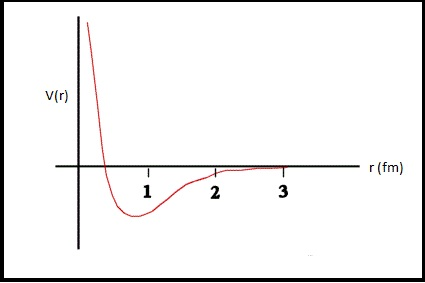
\includegraphics[width=4cm,height=3cm]{Strong_Force.jpg}
\end{center}
\alert{A practice model for the nuclear force should include all these features}. These features are created by various mesons.
\end{itemize}
\end{frame}
\subsection{QCD}
\begin{frame}
\frametitle{QCD}
\begin{itemize}
\item QCD (quantum chromodynamics) is the fundamental theory for the strong force. The nuclear force comes from the QCD Lagrangian
\begin{equation}
\mathcal{L}_{QCD} = \sum_{f = u,d,s,c,b,t} \bar{q}_f (i\slashed{D} - m_f )q_f - \frac{1}{4} \mathcal{G}_{\mu \nu,a}\mathcal{G}^{\mu \nu}_a
\end{equation}
\item \alert{This is often not a realistic option}.
\item \structure{Alternatives}
\begin{enumerate}
\item Effective field theories: They respect the symmetries of QCD.
\item \alert{Meson theory}: The degrees of freedom are nucleons (i.e. protons and neutrons) with mediating particles being mesons.\symbolfootnote[2]{Mesons are bosons and composed of a quark anti-quark ($q \bar{q}$). Protons and neutrons are fermions with quark content ($uud$) and ($ddu$) respectively.}
\end{enumerate}
\end{itemize}
\end{frame}
\subsection{Meson theory}
\begin{frame}
\frametitle{Meson theory: Bonn potentials}
\begin{itemize}
\item To model the nuclear force, our group uses the Bonn potentials.
\item These potentials are derived from a relativistic scattering equation and describe the force between two interacting nucleons as taking place through the \alert{exchange} of \alert{one} \alert{boson} i.e. \alert{OBE}.
\item The use of Feynman diagrams/rules \alert{aid} in calculating the potential. The OBE Feynman diagram is shown below
\begin{figure}[!h]
\centering
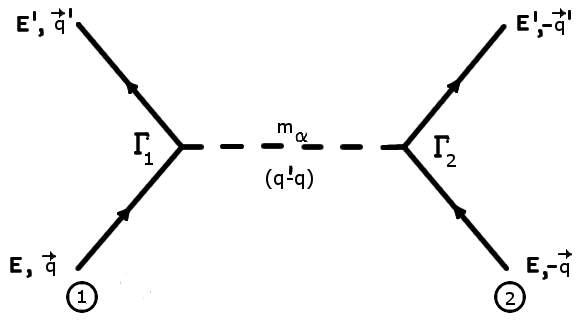
\includegraphics[width=3cm,height=2cm]{feynman.jpg}
\hspace{1cm}
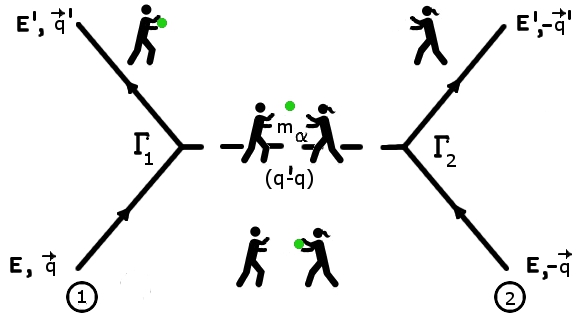
\includegraphics[width=3cm,height=2cm]{feynman_explain.jpg}
\caption{\scriptsize{Left frame: Feynman diagram representing a OBE contribution to nucleon-nucleon scattering in the c.m. frame. Solid lines denote nucleons, the dashed line a meson with mass $m_\alpha$. Right frame: Simple analogy of of Feynman diagram.}}
\end{figure}
\item Additionally, free parameters are constrained using data from nucleon-nucleon scattering and the nucleon-nucleon bound state of Deuteron.
\end{itemize}
\end{frame}
\begin{frame}
\frametitle{Meson theory: Feynman amplitude}
The Feynman diagram on the last slide corresponds to the amplitude $\mathcal{M}_\alpha$ in analytical form
\begin{equation}
\mathcal{M}_\alpha = \frac{ \bar{u} \rb{\bvec{q}_1^\prime,\lambda_1^\prime} \Gamma_1 u \rb{\bvec{q}_1,\lambda_1} P_\alpha \bar{u} \rb{-\bvec{q}_2^\prime,\lambda_2^\prime} \Gamma_2 u \rb{-\bvec{q}_2,\lambda_2} }{ (q^\prime - q)^2 - m^2_\alpha }
\end{equation}
$u$ is a $2 \times 4$ Dirac spinor (helicity ket) and is a solution to the Dirac equation. In block matrix form\symbolfootnote[2]{If $\bvec{q}$ is chosen to lie along the z-axis and $\bvec{q}^\prime$ to lie in the xy-plane then $\ket{\lambda_1},\ket{\lambda_2}=\chi_{\lambda_1}, \chi_{-\lambda_2}$ respectively while $\ket{\lambda_1^\prime},\ket{\lambda_2^\prime}=\exp \rb{-\frac{i}{2}\sigma_2 \theta} \chi_{\lambda_1^\prime}, \exp \rb{-\frac{i}{2}\sigma_2 \theta} \chi_{-\lambda_2^\prime}$ respectively. $\chi_\lambda$ is a usual 2 component Pauli spinor and $\theta$ is the scattering angle (i.e. the axial angle).}
\begin{equation}
u \rb{\bvec{q},\lambda_1} = \sqrt{\frac{E_q+m}{2m}}
\begin{pmatrix}
\mathbbm{1}\\
\frac{2 \lambda_1 \abs{\bvec{q}}}{E_q+m}
\end{pmatrix}
\ket{\lambda_1}
\end{equation}
\begin{equation}
u \rb{-\bvec{q},\lambda_2} = \sqrt{\frac{E_q+m}{2m}}
\begin{pmatrix}
\mathbbm{1}\\
\frac{2 \lambda_2 \abs{\bvec{q}}}{E_q+m}
\end{pmatrix}
\ket{\lambda_2}
\end{equation}
\scriptsize{Where $E_q=\sqrt{m^2+\abs{\bvec{q}}^2}$, $\bar{u}=u^\dagger \gamma^0$, and the corresponding meson Lagrangian determines $P_\alpha$ and $\Gamma_{1 \rb{2}}$.}
\vspace{0.15cm}
\end{frame}
\begin{frame}
\frametitle{Meson theory: Lagrangian's}
Guided by symmetry principles, simplicity, and physical intuition, the most commonly used interaction Lagrangian's are\symbolfootnote[2]{Unless stated otherwise, we use the conventions and notations of Bjorken and Drell. For example: $\hbar=c=1$, $\gamma^0=\bigl(\begin{smallmatrix}1&0\\0&-1\end{smallmatrix}\bigr)$, $\gamma^k=\bigl(\begin{smallmatrix}0&\sigma^k\\-\sigma^k&0\end{smallmatrix}\bigr)$ with $\sigma^k$ the usual Pauli matrices, $\gamma_5=\gamma^5=\bigl(\begin{smallmatrix}0&1\\1&0\end{smallmatrix}\bigr)$, $\sigma^{\mu \nu}=\rb{i/2} \left[\gamma^\mu, \gamma^\nu \right]$, the metric tensor $g$ is $g_{00}=1$ $g_{kk}=-1$ $g_{\mu \neq \nu}=0$, and Einstein summation notation is used.}
\begin{equation}
\mathcal{L}_{pv} = -\frac{f_{ps}}{m_{ps}} \bar{\psi} \gamma^5 \gamma^\mu \psi \partial_{\mu} \phi^{\rb{ps}}
\end{equation}
\begin{equation}
\mathcal{L}_{s} = g_{s} \bar{\psi} \psi \phi^{\rb{s}}
\end{equation}
\begin{equation}
\mathcal{L}_{v} = -g_{v} \bar{\psi} \gamma^\mu \psi \phi_\mu^{\rb{v}} - \frac{f_v}{4m} \bar{\psi} \sigma^{\mu \nu} \psi \rb{\partial_\mu \phi_\nu^{\rb{v}} - \partial_\nu \phi_\mu^{\rb{v}}}
\end{equation}
\scriptsize{Where $\psi$ denotes the nucleon Dirac spinor field, while $\phi^{\rb{ps}}$,$\phi^{\rb{s}}$,$\phi_\mu^{\rb{v}}$ are the pseudo-scalar, scalar, and vector boson fields, respectively. Everything else is a constant.}
\end{frame}
\begin{frame}
\frametitle{Meson theory: Scalar (s) potential ($\sigma$ and $\rho$ mesons)}
\begin{itemize}
\item $\Gamma_{1 \rb{2}} = i$ times the Lagrangian stripped off the fields 
\begin{equation}
\mathcal{L}_{s} = g_{s} \bar{\psi} \psi \phi^{\rb{s}} \Rightarrow
\end{equation}
\begin{equation}
\Gamma_{1\rb{2}} = g_{s} i \Rightarrow
\end{equation}
\begin{equation}
\mathcal{M}_{s} = \frac{ g_{s}^2 \bar{u} \rb{\bvec{q}_1^\prime,\lambda_1^\prime} i u \rb{\bvec{q}_1,\lambda_1} P_{s} \bar{u} \rb{-\bvec{q}_2^\prime,\lambda_2^\prime} i u \rb{-\bvec{q}_2,\lambda_2} }{ (q^\prime - q)^2 - m^2_{s} }
\end{equation}
\item The potential\symbolfootnote[2]{$V_{s}=\braket{\bvec{q}^\prime \lambda_1^\prime \lambda_2^\prime|V_{s}|\bvec{q} \lambda_1 \lambda_2}$ and $P_{s} = i$. Additionally, $\delta$ has isospin $1$ which introduces an extra factor $\bvec{\tau}_1 \cdot \bvec{\tau}_2$, where $\bvec{\tau}_{1 \rb{2}}$ are the usual Pauli spin matrices. Also, $\bar{u}=u^\dagger \gamma^0$. } is $i$ times $\mathcal{M}$
\begin{equation}
V_{s} = \frac{ g_{s}^2 \bar{u} \rb{\bvec{q}_1^\prime,\lambda_1^\prime} u \rb{\bvec{q}_1,\lambda_1} \bar{u} \rb{-\bvec{q}_2^\prime,\lambda_2^\prime} u \rb{-\bvec{q}_2,\lambda_2} }{ (q^\prime - q)^2 - m^2_{s} }
\end{equation}
\end{itemize}
\end{frame}
\begin{frame}
\frametitle{Meson Theory: Determination of constants}
\begin{itemize}
\item Two nucleon scattering is described by the BS equation. One possible three-dimensional reduction is the Blankenbecler and Sugar (BbS) equation
\begin{equation}
\hat{\mathcal{M}}\rb{\bvec{q}^\prime,\bvec{q}} = \hat{V} \rb{\bvec{q}^\prime,\bvec{q}} + \int \frac{ \hat{V} \rb{\bvec{q}^\prime,\bvec{q}}}{ \rb{2 \pi}^3} \frac{m}{\bvec{q}^2-\bvec{k}^2 +i \epsilon} \hat{\mathcal{M}}\rb{\bvec{k}^\prime,\bvec{q}} d^3k
\end{equation}
Where, $\hat{V} \rb{\bvec{q}^\prime,\bvec{q}}=\rb{\frac{m}{E_{q^\prime}}}^{1/2} V \rb{\bvec{q}^\prime,\bvec{q}}  \rb{\frac{m}{E_{q}}}^{1/2}$ and similarly for $\hat{\mathcal{M}}\rb{\bvec{q}^\prime,\bvec{q}}$.
\item Use experimental scattering data from Deuteron (i.e. experimental value for $\hat{\mathcal{M}}\rb{\bvec{q}^\prime,\bvec{q}}$) along with the BbS equation to determine constants. 
\end{itemize}
\end{frame}
\begin{frame}
\frametitle{Meson theory: Final form for the potential}
\begin{itemize}
\item The use of the BbS equation results in $\rb{q^\prime - q}^2=-\rb{\bvec{q}^\prime-\bvec{q}}^2$.
\item A form factor $F_\alpha \left[ \rb{\bvec{q}^\prime - \bvec{q}^2} \right]$ term is included at each vertex to simulate the short range of the nuclear force.
\item The final version of the scalar potential is written in literature as
\begin{eqnarray}
V_{s}&=&-\frac{g^2_{s}}{\rb{2 \pi}^3} \sqrt{\frac{m}{E_{q^\prime}}} \sqrt{\frac{m}{E_{q}}} \rb{F_s \left[ \rb{\bvec{q}^\prime - \bvec{q}^2} \right] }^2 \nonumber \\
&\times&\frac{\bar{u} \rb{\bvec{q}_1^\prime,\lambda_1^\prime} u \rb{\bvec{q}_1,\lambda_1} \bar{u} \rb{\bvec{-q}_2^\prime,\lambda_2^\prime} u \rb{\bvec{-q}_2,\lambda_2}}{(\bvec{q}^\prime - \bvec{q})^2 + m^2_{s}}
\end{eqnarray}
\item Similar results hold for the pesudo-scalar ($\pi$, $\eta$) and vector ($\omega$, $\rho$) mesons.\symbolfootnote[2]{See for example, \emph{The Bonn Meson-Exchange Model for the Nucleon-Nucleon Interaction, R. Machleidt et al., Phys. Rep. 149, (1987).}}
\item The resulting Bonn potential is the sum of the OBE potentials.
\begin{equation}
V = \sum_{\alpha=\rb{\pi,\eta}_{ps},\rb{\delta,\sigma}_{s},\rb{\rho,\omega}_{v}} V_{\alpha}
\end{equation}
\end{itemize}
\end{frame}
\section{DBHF}
\subsection{Overview}
\begin{frame}
\frametitle{DBHF: Overview}
\begin{itemize}
\item With a quantitative two-body interaction and the chosen many-body theory, namely Dirac-Brueckner-Hartree-Fock (DBHF), we are ready to go into the many-body system. Our playground is \alert{nuclear matter}\symbolfootnote[1]{When we speak of nuclear matter we mean an infinite uniform system of nucleons interacting via the strong force without electromagnetic interactions. This hypothetical system is supposed to approximate conditions in the interior of a heavy nucleus.} with different concentrations of protons and neutrons. This is commonly referred to as \alert{isospin-asymmetric nuclear matter (IANM)}.
\item The essential point of the Dirac-Brueckner-Hartree-Fock (DBHF) approach is to use the Dirac equation for the single-particle motion in nuclear matter\symbolfootnote[2]{Feynman slash notation is used, i.e. $\slashed{p}=\gamma_\mu p^\mu$.}
\begin{equation}
\rb{ \slashed{p} - m_i - U_i } u_i \rb{\bvec{p},\lambda} = \bvec{0}
\end{equation}
\begin{equation}
i=n,p \text{   \emph{For n = neutron and p = proton.} }
\end{equation}
With $U_i=U_{S,i}+\gamma^0 U^0_{V,i}$. $U_{S,i}$ is an attractive scalar and $U^0_{V,i}$ the time component of a repulsive vector field. $m_i$ is the free space neutron(proton) mass.
\end{itemize}
\end{frame}
\subsection{DBHF details}
\begin{frame}
\frametitle{DBHF}
\begin{itemize}
\item Positive energy solutions to the Dirac equation are
\begin{equation}
\tilde{u}_i \rb{\bvec{p},\lambda} =
\sqrt{\frac{ \tilde{E}_{\bvec{p},i} + \tilde{m_i}}{2 \tilde{m_i}} }
\begin{pmatrix}
\mathbbm{1}\\
\frac{\bvec{\sigma} \cdot \bvec{p}}{\tilde{E}_{\bvec{p},i} + \tilde{m_i}}
\end{pmatrix}
\chi_\lambda
\label{helicity} 
\end{equation}
with, $\tilde{m}_i=m_i+U_{S,i}$, $\tilde{E}_{\bvec{p},i}=\sqrt{\tilde{m_i}^2 + \bvec{p}^2}$ and $\chi_\lambda$ a conventional Pauli spinor.
\item From this we can compute the $U_i \rb{p}$ matrix elements\symbolfootnote[2]{Where $\ket{\bvec{p}}$ is a helicity ket defined in Eq. \ref{helicity} and $\bra{\bvec{p}} = \bar{\tilde{u}}$.}
\begin{equation}
U_i \rb{p} = \frac{\tilde{m}_i}{\tilde{E}_i} \braket{\bvec{p}|U_i \rb{p}|\bvec{p}} = \frac{\tilde{m}_i}{\tilde{E}_i} U_{s,i} + U^0_{V,i}
\end{equation}
\end{itemize}
\end{frame}
\begin{frame}
\frametitle{DBHF: continued}
The Thompson equation is an alternative to the Bbs equation\symbolfootnote[2]{Definitions: $\bvec{P}=\bvec{k}_1 + \bvec{k}_2$, $\bvec{K}=\frac{\bvec{k}_1-\bvec{k}_2}{2}$, $\tilde{\epsilon}_{ij}=\tilde{e}_i \rb{\bvec{P},\bvec{K}}+\tilde{e}_j \rb{\bvec{P},\bvec{K}}$, and $\rb{\tilde{\epsilon}_{ij}}_0$ is the starting energy.}
\begin{eqnarray*}
\tilde{G}_{ij} \rb{\bvec{q}^\prime,\bvec{q},\bvec{P},\rb{\tilde{\epsilon}_{ij}}_0}&=&\tilde{V}_{ij} \rb{\bvec{q}^\prime,\bvec{q}} \\
&+&\int \frac{d^3k \tilde{V}_{ij} \rb{\bvec{q}^\prime,\bvec{k}} }{\rb{2 \pi}^3} \frac{\tilde{m}^2 Q_{ij} \rb{\bvec{k},\bvec{P}}}{ \rb{\tilde{\epsilon}_{ij}}_0 \tilde{\epsilon}_{ij} \rb{\bvec{P},\bvec{k}} } \tilde{G} \rb{\bvec{k},\bvec{q},\bvec{P},\rb{\tilde{\epsilon}_{ij}}_0}
\end{eqnarray*}
\begin{equation}
ij = nn,pp,np \text{   \emph{For n = neutron and p = proton.} }
\end{equation}
From this we obtain $U_i \rb{p}$\symbolfootnote[1]{$k^i_F$ is the Fermi momentum of the neutron(proton). For IANM the neutron(proton) density is related to the neutron(proton) Fermi momentum by $\rho_i={\rb{k^i_F}^3}/{\rb{3 \pi^2}}$.}
\begin{equation}
U_i \rb{p} = \sum_{j=n,p} \sum_{p^\prime \leq k^j_F} G_{ij} \rb{\bvec{p},\bvec{p}^\prime}
\end{equation}
\end{frame}
\begin{frame}
\frametitle{DBHF: summary}
In summary
\begin{equation}
U_i \rb{p} = \sum_{j=n,p} \sum_{p^\prime \leq k^j_F} G_{ij} \rb{\bvec{p},\bvec{p}^\prime}
\label{UG}
\end{equation}
\begin{equation}
U_i \rb{p} = \frac{\tilde{m}_i}{\tilde{E}_i} U_{s,i} + U^0_{V,i}
\label{UC}
\end{equation}
Values for\symbolfootnote[2]{Note, $\tilde{m}_i-m=U_{s,i}$} $\tilde{m}_i \Rightarrow U_{s,i}$, and $U^0_{V,i}$ are chosen and from them $G_{ij} \rb{\bvec{p},\bvec{p}^\prime}$ is calculated. Thus, we obtain $U_i \rb{p}$. Then we evaluate $U_i \rb{p}$ at two arbitrary momentums e.g. $U_i \rb{p_1}$ and $U_i \rb{p_2}$. Finally, using these points in Eq. \ref{UC}, we compute updated values for $\tilde{m}_i$, and $U^0_{V,i}$. These updated values are then used to compute an updated value for $G_{ij} \rb{\bvec{p},\bvec{p}^\prime}$. This procedure is repeated until a desired accuracy is achieved.   
\end{frame}
\subsection{EoS}
\begin{frame}
\frametitle{EoS: Formulas}
\begin{itemize}
\item \alert{The equation of state (EoS) is the output of our DBHF calculations}. Using results from the previous slides we can calculate the (average) energy per neutron or proton in nuclear matter ($\bar{e}_i$). This is equal to the average kinetic energy\symbolfootnote[1]{The kinetic energy is $T_i=\rb{\tilde{m}_i / \tilde{E}_i} \braket{\bvec{p}|\bvec{\gamma} \cdot \bvec{p}+m_i|\bvec{p}}=\rb{ m_i \tilde{m}_i+\bvec{p}^2} / \tilde{E}_i$.} $\langle T_i \rangle$ plus the average potential energy $\langle U_i \rangle$
\begin{equation}
\bar{e}_i = \frac{1}{A} \langle T_i \rangle + \frac{1}{2A} \langle U_i \rangle - m_i
\end{equation}
\item This result leads us to the EoS ($\bar{e}$). \alert{The EoS is the (average) energy per nucleon as a function of the neutron and proton density} $\bar{e} \rb{\rho_n,\rho_p}$
\begin{equation}
\bar{e} \rb{\rho_n,\rho_p} = \frac{\rho_n \bar{e}_n + \rho_p \bar{e}_p}{\rho}
\end{equation}
\item To a very good degree of approximation, the EoS is written as\symbolfootnote[2]{$\rho=\rho_n+\rho_p$ and $\alpha$ is the neutron excess parameter defined as $\alpha=\frac{\rho_n-\rho_p}{\rho}$.}
\begin{equation}
\small{
\bar{e} \rb{\rho,\alpha} \approx \bar{e} \rb{\rho, \alpha=0} + \left[ \bar{e} \rb{\rho,\alpha=1} - \bar{e} \rb{\rho,\alpha=0} \right]\alpha^2 = e_0 \rb{\rho} + e_{sym} \rb{\rho} \alpha^2
}
\end{equation}
\end{itemize}
\end{frame}
\begin{frame}
\frametitle{EoS: Plots}
\begin{figure}[!h]
\centering
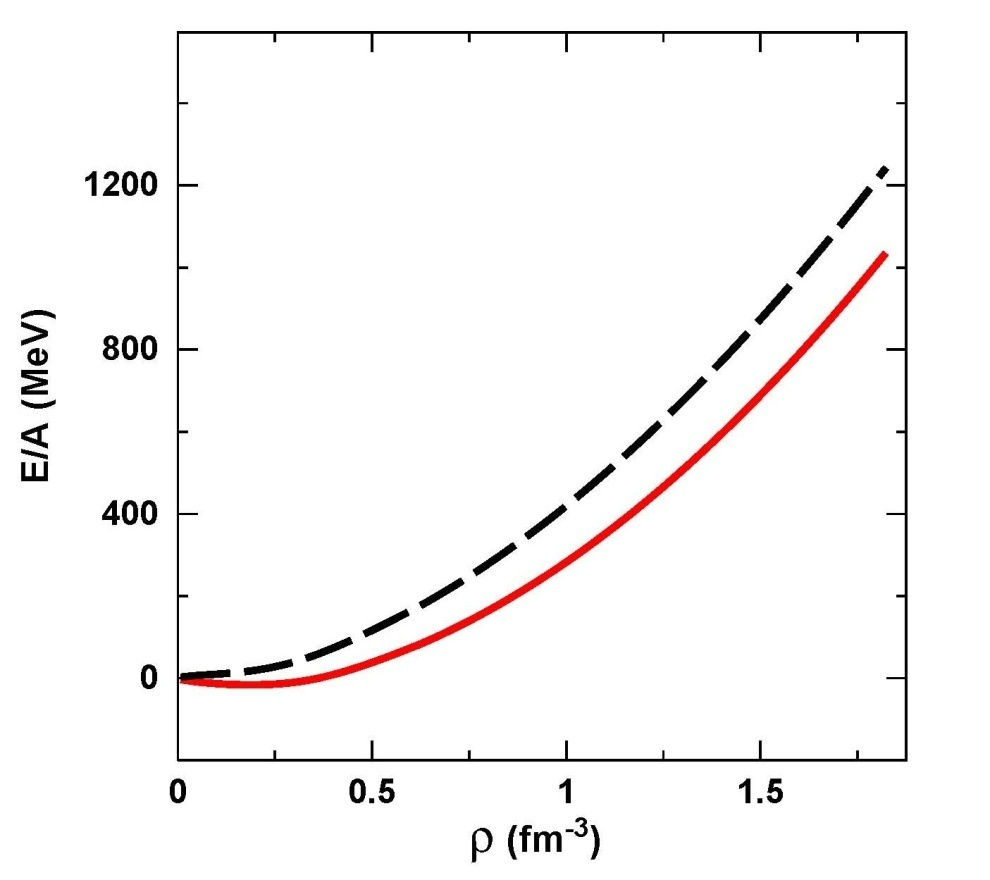
\includegraphics[width=3.5cm,height=2cm]{eos.jpg}
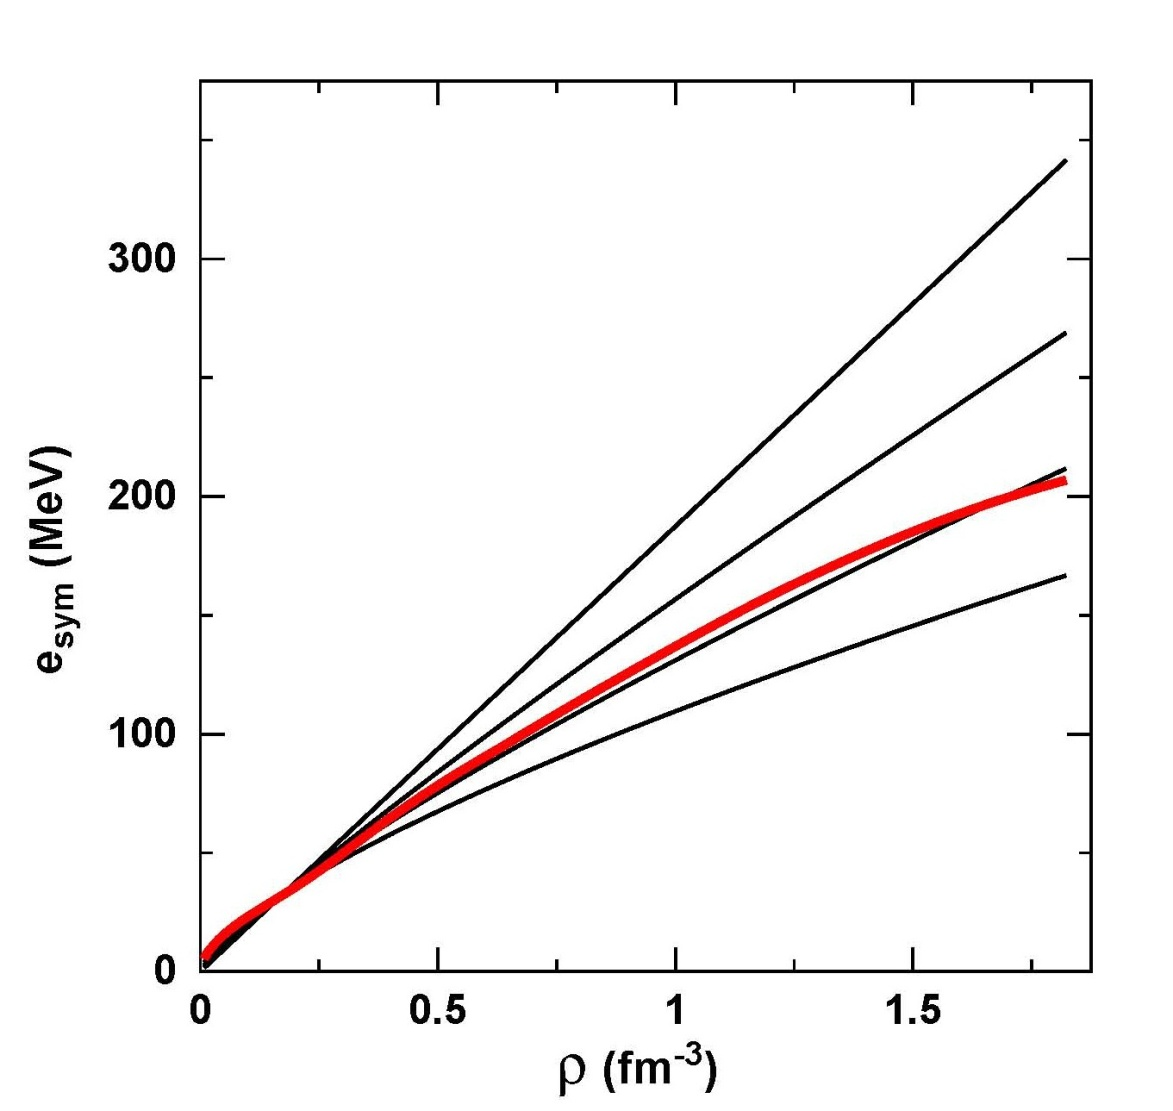
\includegraphics[width=3.5cm,height=2.1cm]{esym.jpg}
\caption{\scriptsize{Left frame: DBHF predictions for the EoS of symmetric matter i.e. $\alpha=0$ (solid red) and and neutron matter i.e. $\alpha = 1$ (dash black). Right frame: DBHF predictions for the symmetry energy (solid red) compared with various phenomenological parameterizations (dashed black), as explained below. See: \emph{A microscopic equation of state for neutron-rich matter and its effect on neutron star properties, Francesca Sammarruca, p. 180-212, (2011).}}}
\end{figure}
\begin{itemize}
\item \footnotesize{(Left frame) The predicted saturation density and energy for symmetric matter are $0.185 \text{ fm}^{-3}$ and $-16.14 \text{ MeV}$ respectively. Our predictions of the EoS (for both symmetric and asymmetric matter), are well within available constraints. However, more and better constraints are needed especially at high density, where model dependence is largest.}
\item \footnotesize{(Right frame) The various black dashed curves were obtained with the simple parameterization $e_{sym}=C \rb{\rho/\rho_0}^\gamma$ for $\gamma$ from $0.7$ to $0.1$ in steps of $0.1$ and $C \approx 32 \text{ MeV}$. \alert{Clearly, this reflects our limited knowledge of the symmetry energy}.}
\end{itemize}
\end{frame}
\subsection{}
\begin{frame}
\begin{center}

\includegraphics[width=5.6cm,height=8cm]{clown.jpg}
\end{center}
\end{frame}
\section{Predictions}
\subsection{BE calculations}
\begin{frame}
\frametitle{BE calculations}
\begin{itemize}
\item Allows us to compute density functions and binding energies (BE), \alert{both of which are observables}.
\item \alert{Density functions are used as input to calculate other observables}.
To calculate the BE $B$ a simple liquid drop model is used. It's analogous to the Bethe-Weizs\"{a}cker relation\symbolfootnote[2]{Recall, the EoS ($\bar{e}$) is a function of the proton $\rho_p \rb{\bvec{r}}$ and neutron $\rho_n \rb{\bvec{r}}$ density. Also, the total density is $\rho \rb{\bvec{r}}=\rho_p \rb{\bvec{r}} + \rho_n \rb{\bvec{r}}$ and $f_0= 70 \text{ MeV} \cdot \text{fm}^{-5}$.}
\item \alert{Notice the EoS is used as input for the calculation}.
\begin{eqnarray}
-B&=&\int \bar{e} \rb{ \rho_p \rb{\bvec{r}},\rho_n \rb{\bvec{r}} } \rho \rb{\bvec{r}} d^3 r + f_0 \int \abs{\nabla \rho \rb{\bvec{r}}}^2 d^3 r \nonumber \\
&&+\frac{e^2}{8 \pi \epsilon_o} \iint \frac{\rho_p \rb{\bvec{r}} \rho_p \rb{\bvec{r}^\prime}}{\abs{\bvec{r}-\bvec{r}^\prime}}d^3 r d^3 r^\prime
\end{eqnarray}
\end{itemize}
\end{frame}
\begin{frame}
\frametitle{BE: Spherical and Azimuthal symmetry}
\begin{itemize}
\item Pick a proton/neutron density function. The density function will depend on parameters. We usually use a two-parameter Fermi function. For spherical symmetry
\begin{equation}
\rho_i \rb{r} = \frac{N_i}{1+\exp \rb{\frac{r-R_i}{c_i}}}
\end{equation}
\item In preparation for calculations of deformed nuclei, we have extended our energy functional to include the possibility of angular dependence. \alert{This is work in progress}.
\begin{equation}
\rho_i \rb{r,\theta} = \frac{N_i}{1+\exp \rb{\frac{r-R_i \rb{\theta}}{c_i}}}
\end{equation}
where $i=n,p$ and $N_i$ is a normalization constants. 
\item The parameters $R_i$($R_i \rb{\theta}$) and $c_i$ are to be determined by maximizing the binding energy.
\end{itemize}
\end{frame}
\begin{frame}
\frametitle{BE results: Density functions}
\begin{figure}[!h]
\centering
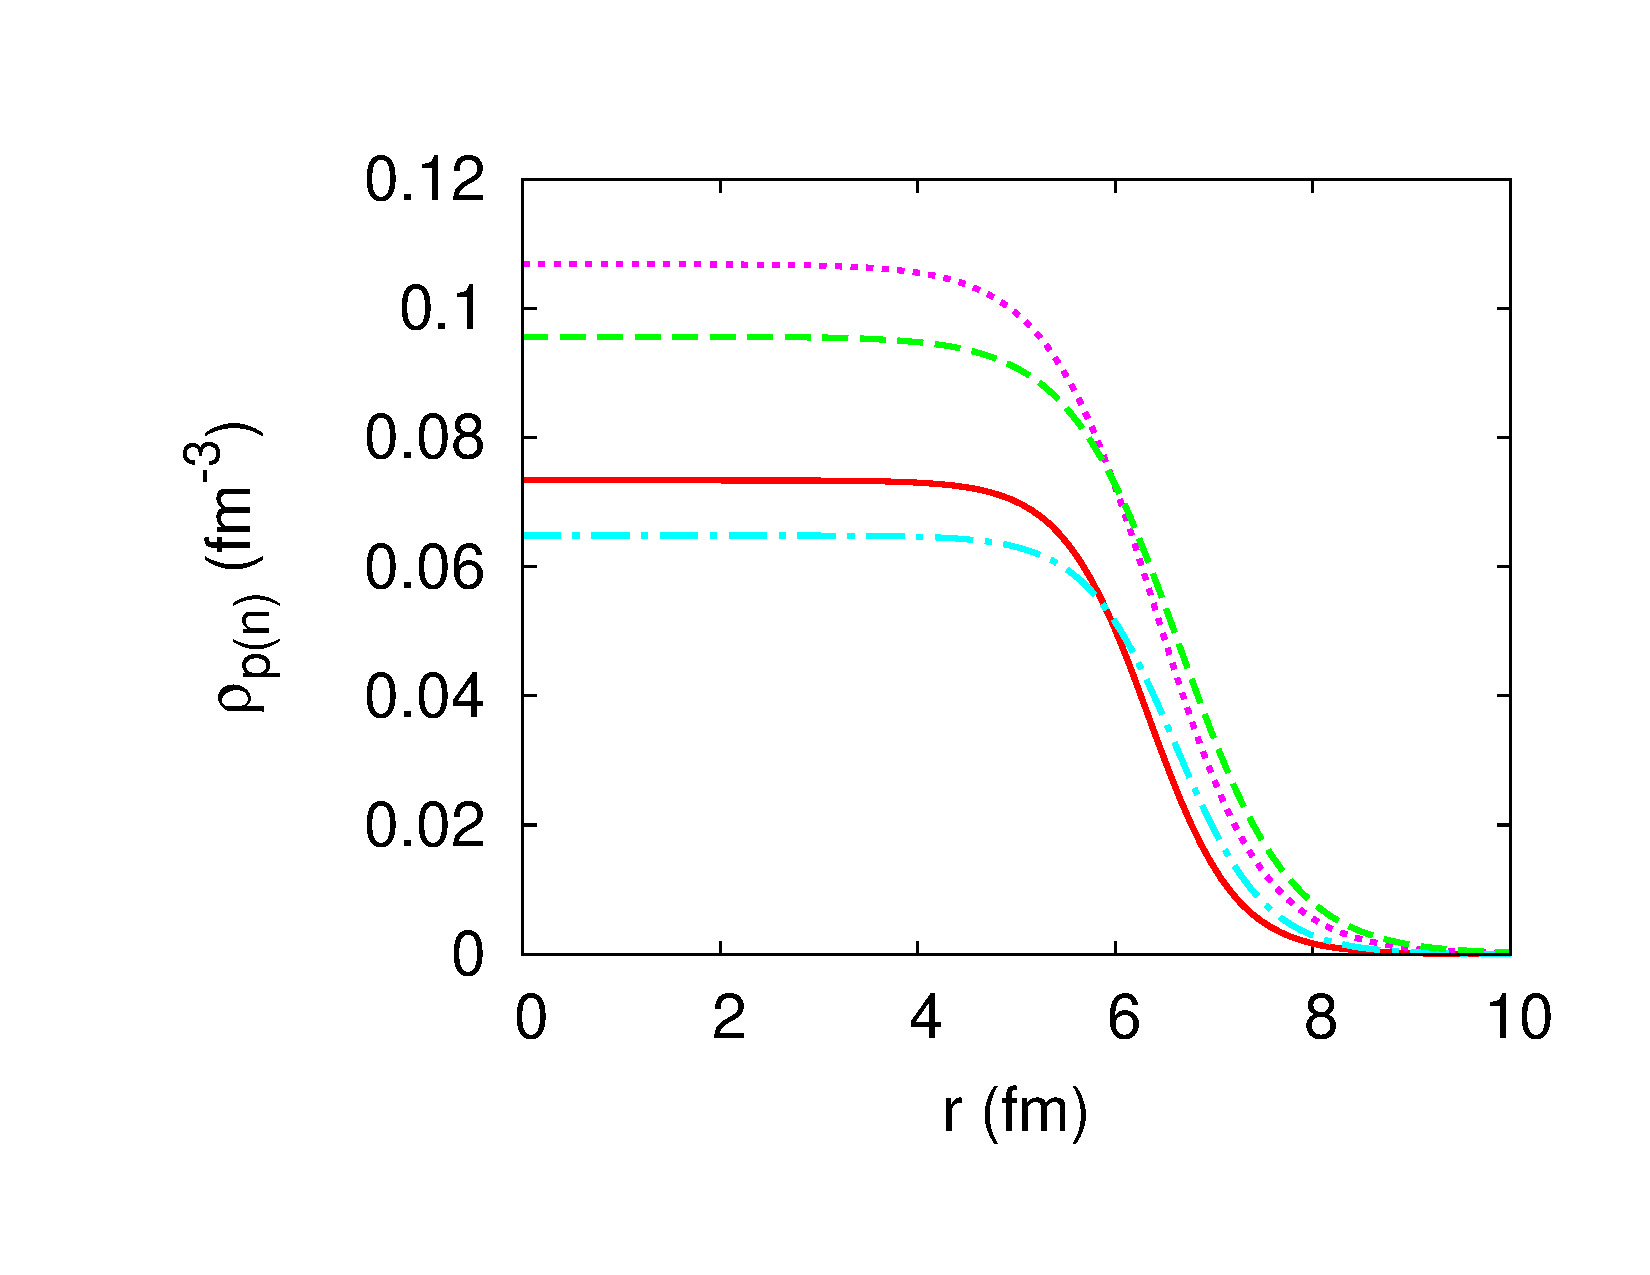
\includegraphics[width=5.5cm,height=3.5cm]{208Pb_rho_Bonn.pdf}
\hspace{1cm}
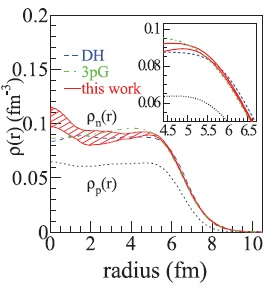
\includegraphics[width=2.6cm,height=2.6cm]{rho_exp.jpg}
\caption{\scriptsize {Left frame: $^{208}$Pb density functions used to describe the proton (Bonn A: solid red curve and Bonn B: dash dotted blue curve) and the neutron (Bonn A: dotted pink curve and Bonn B: dashed green curve) densities. Right frame: Experimentally measured $^{208}$Pb neutron and proton density function. Experimental results from \emph{J. Zenihiro et al., Phys. Rev. C 82 044611, (2010).} }}
\end{figure}
\end{frame}
\begin{frame}
\frametitle{BE results: RMS radii and neutron skins}
\begin{itemize}
\item From the neutron/proton density functions we can calculate and compare RMS radii $\langle r^2_{pt} \rangle_i^{1/2}$ and neutron skins $S_n$
\begin{equation}
\langle r^2_{pt} \rangle_i^{1/2} = \sqrt{\frac{4 \pi}{N_i} \int_0^\infty r^4 \rho_i \rb{r} dr }
\end{equation}
For $i=n,p$ and $N_i$ the neutron(proton) number.
\begin{equation}
S_n = \langle r^2_{pt} \rangle_n^{1/2}-\langle r_{pt} \rangle_p^{1/2}
\end{equation}
\end{itemize}
\end{frame}
\begin{frame}
\frametitle{RMS radii and neutron skins results}
\begin{table}[!h]
\caption{Theoretical and experimental: proton/neutron RMS radii, neutron skins and binding energies for $^{208}$Pb. All values in fm unless stated otherwise.}
\centering
\begin{tabular}{cccccc}
\hline\hline
& $\langle r^2_{pt} \rangle_n^{1/2}$ & $\langle r^2_{pt} \rangle_p^{1/2}$ & $S_n$ & $B$ (MeV) &\\ \hline
\multirow{1}{*}{Theo. Bonn A}& $5.36$ & $5.17$ & $0.19$ & $8.36$ &\\
\multirow{1}{*}{Theo. Bonn B}& $5.56$ & $5.39$ & $0.17$ & $7.19$ &\\
\multirow{1}{*}{Exp.\symbolfootnote[2]{RMS radii and neutron skins: J. Zenihiro et al., Phys. Rev. C 82, 044611 (2010).}\symbolfootnote[1]{BE: United States National Nuclear Data Center, Brookhaven National Laboratory, ``Nudat 2.3,'' online (2007).}}& $5.653^{+0.054}_{-0.063}$ & $5.442(2)$ & $0.211^{+0.054}_{-0.063}$ & $7.87$ &\\
\hline\hline
\end{tabular}
\end{table}
\end{frame}
\subsection{Reaction cross section}
\begin{frame}
\frametitle{Total reaction cross section}
The total reaction cross section $\sigma_R$ is of fundamental importance in theoretical and experimental physics
\begin{equation}
\sigma_R = 2 \pi \int_0^\infty \rb{ 1 - T(b) } b db
\end{equation}
\begin{equation}
T(b) = \exp \left[   -\iint f \rb{ \abs{\bvec{r}_T - \bvec{r}_P} } \sum_{\substack{i=n,p\\j=n,p}} \sigma_{ij} \rho^{\rb{T}}_{z,i} \rb{\bvec{r}_T} \rho^{\rb{P}}_{z,j} \rb{ \abs{\bvec{r}_P - \bvec{b}} } d^2 r_T d^2 r_P  \right]
\end{equation}
where $f \rb{ \abs{\bvec{r}_T - \bvec{r}_P} }$ is usually taken to be a Gaussian and $\sigma_{ii}$($\sigma_{ij}$) are the nucleon-nucleon cross sections for scattering of identical(non-identical) nucleons. Also,
\begin{equation}
\rho_{z,i}^{\rb{T}} \rb{\abs{\bvec{r}_T}} = \int \rho_i^{\rb{T}} \rb{ \sqrt{\bvec{r}^2_T + z^2} } dz
\end{equation}
\begin{equation}
\rho_{z,j}^{\rb{P}} \rb{\abs{\bvec{r}_P-\bvec{b}}} = \int \rho_j^{\rb{P}} \rb{ \sqrt{\abs{\bvec{r}_P-\bvec{b}} + z^2} } dz
\end{equation}
\end{frame}
\begin{frame}
\frametitle{Total reaction cross section: Results}
\begin{figure}[!h]
\centering
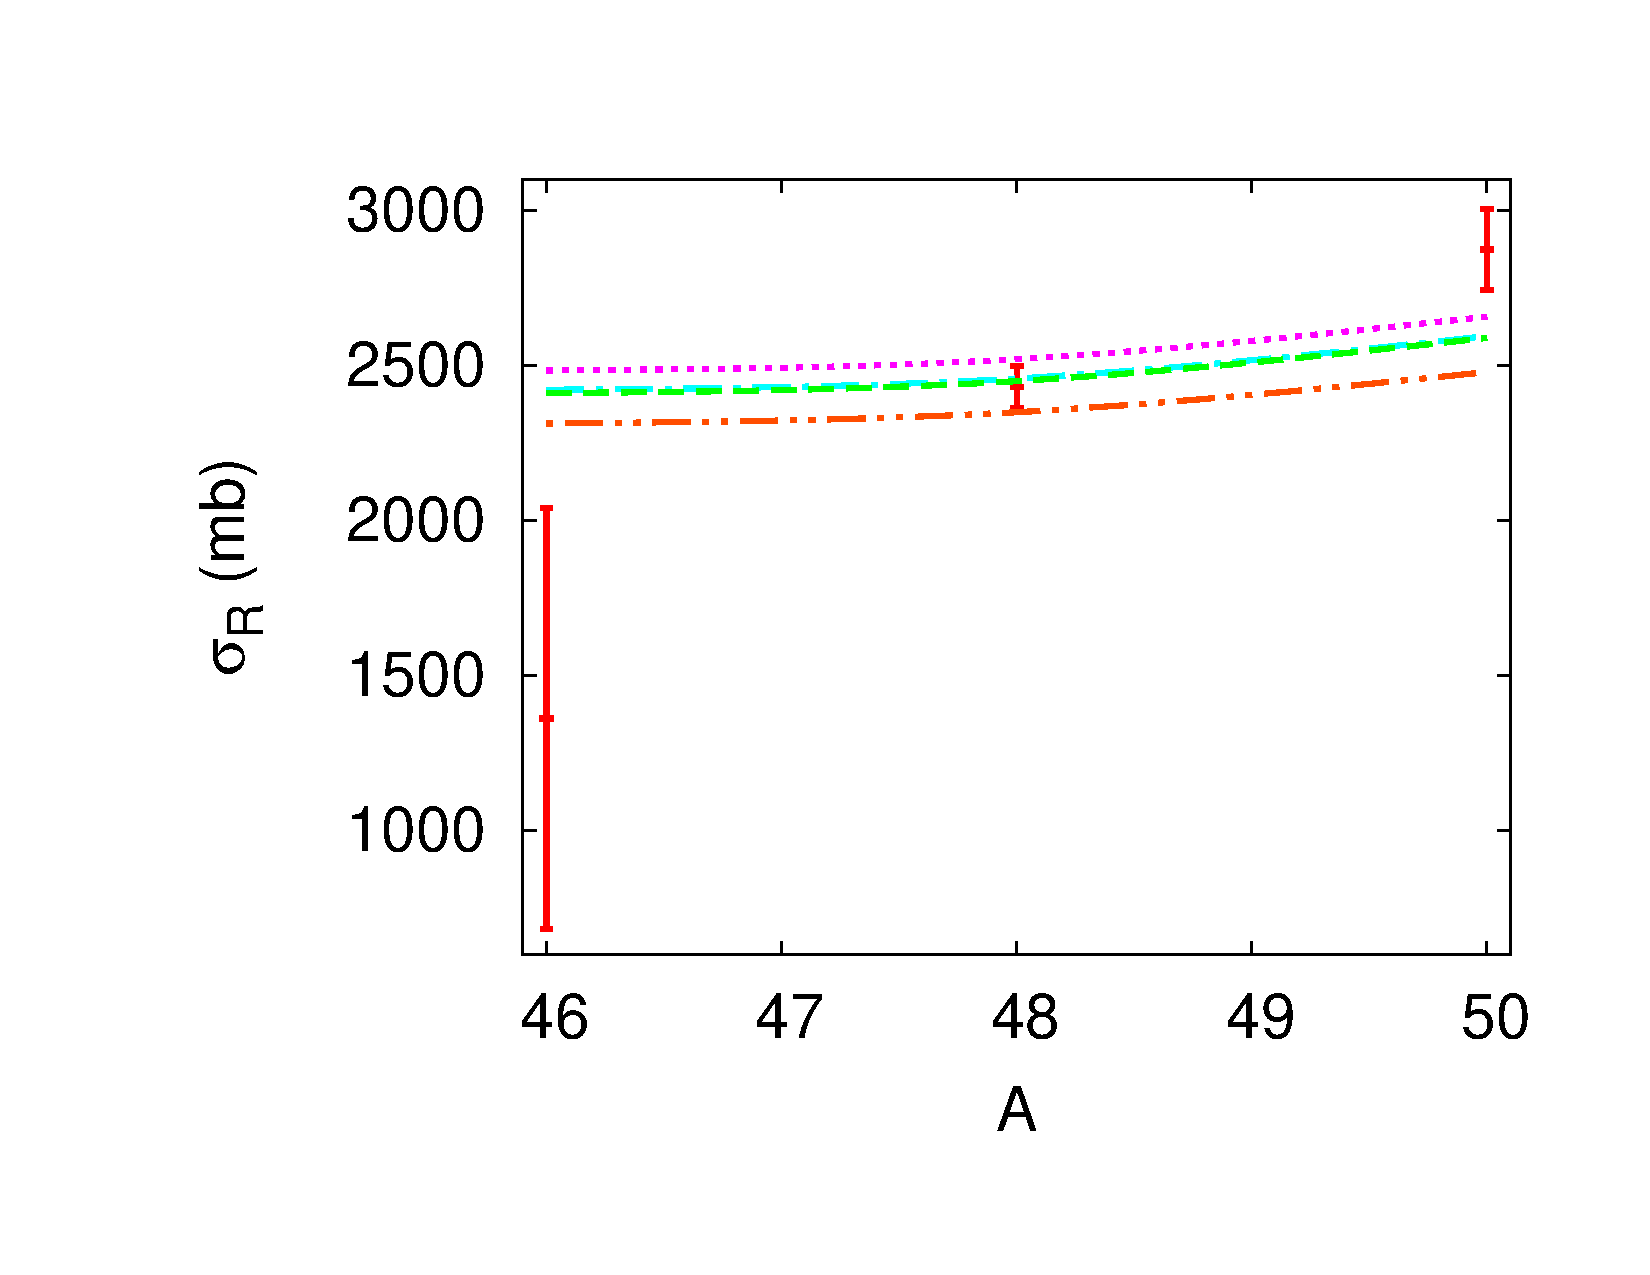
\includegraphics[width=6cm,height=3.7cm]{Ca.pdf}
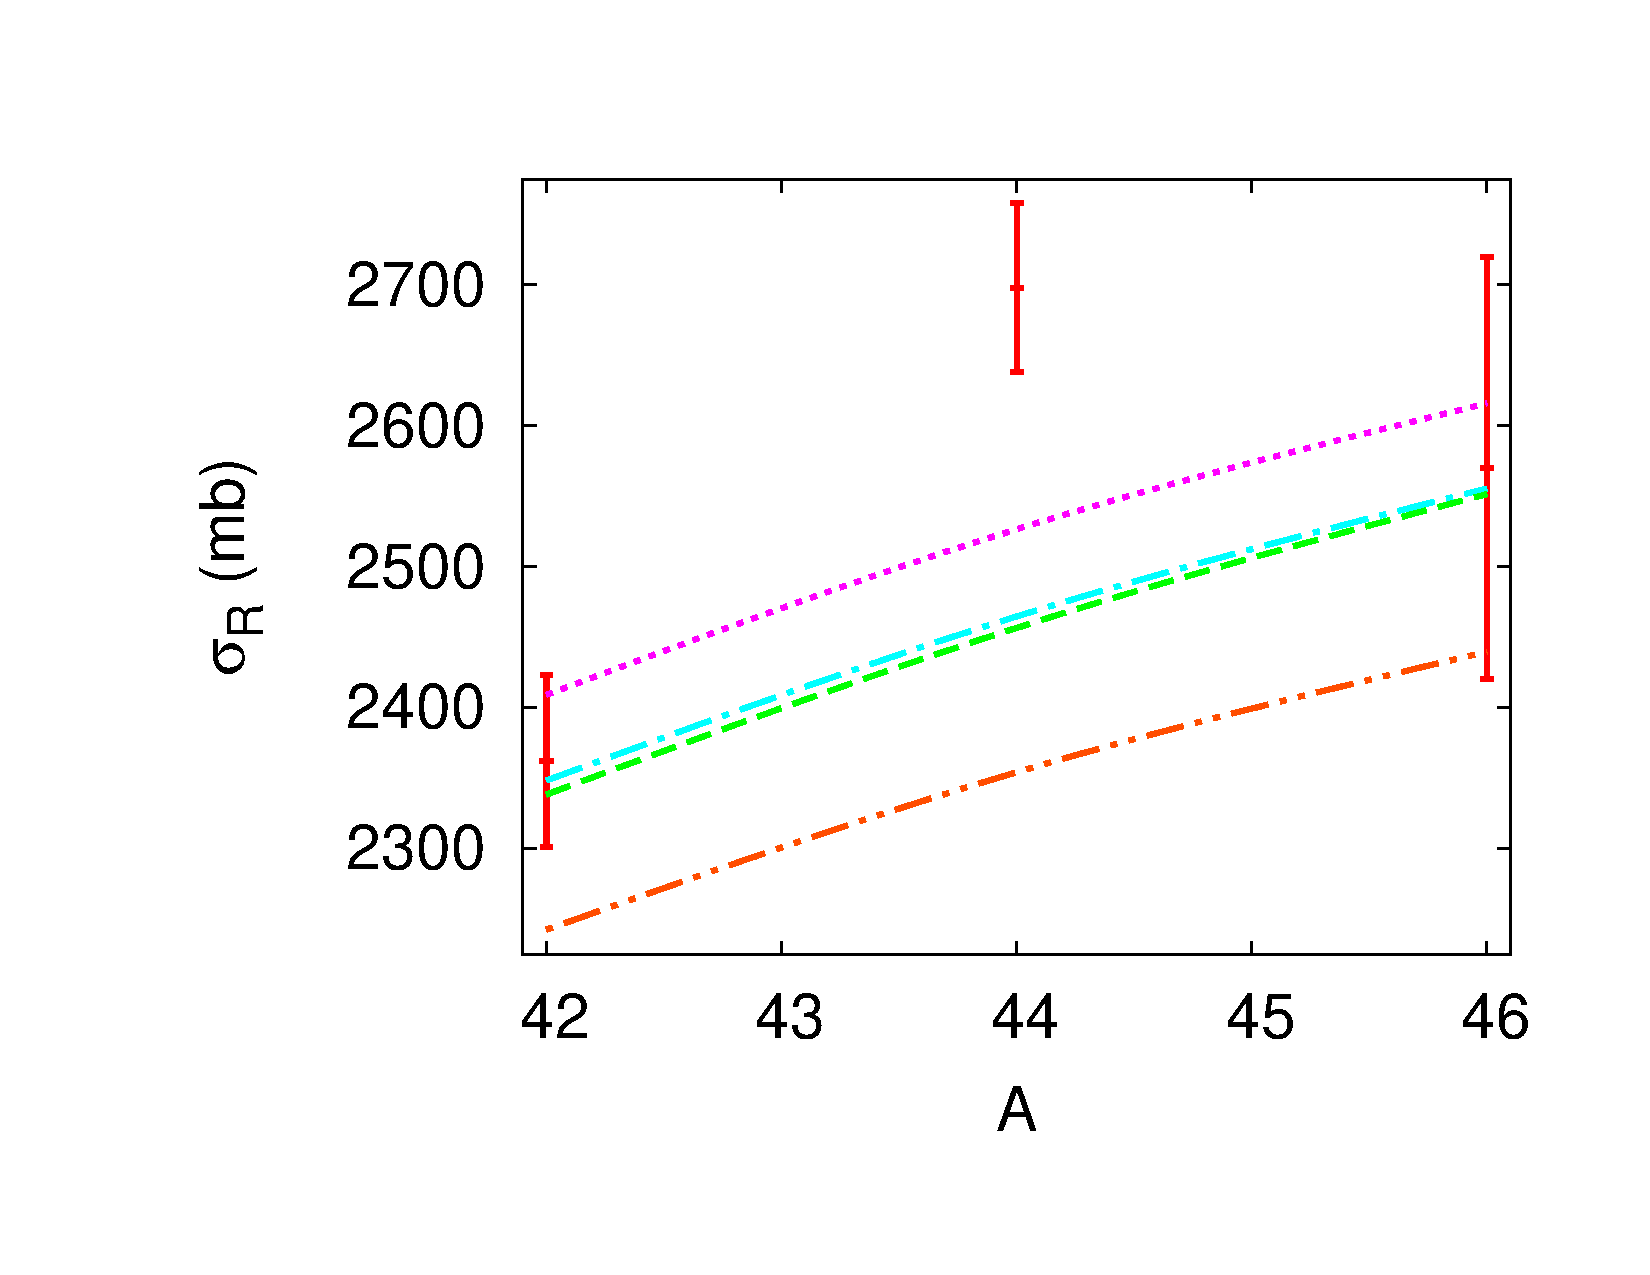
\includegraphics[width=6cm,height=3.7cm]{Ar.pdf}
\caption{Plot of the reaction cross section $\sigma_R$ as a function of the mass number of Calcium isotopes (left frame) and Argon isotopes (right frame). The different curves represent different models we used to calculate $\sigma_R$. Data from: \emph{I. Locot et al., Phys. Rev. C 56, 250 (1997)}.}
\end{figure}
\end{frame}
\subsection{Current work}
\begin{frame}
\frametitle{Current work: Development of an improved effective interaction}
\begin{itemize}
\item \alert{My future plans have a solid foundation is what we have discussed so far}.
\item In our microscopic approach, the effective interaction (a nucleon-nucleon interaction modified by the presence of the nuclear medium), is the solution of the Thompson integral equation
\begin{equation}
\scriptsize{
\tilde{G} \rb{\bvec{q}^\prime,\bvec{q}|\bvec{P},\tilde{z}} = \tilde{V} \rb{\bvec{q}^\prime,\bvec{q}} + \mathcal{P} \int \frac{d^3k \tilde{V} \rb{\bvec{q}^\prime,\bvec{k}} }{\rb{2 \pi}^3} \frac{\tilde{m}^2}{\tilde{E}^2_{\rb{1/2}\bvec{P}+\bvec{k}}} \frac{Q \rb{\bvec{k},\bvec{P}}}{\tilde{z}-2\tilde{E}_{\rb{1/2}\bvec{P}+\bvec{k}}} \tilde{G} \rb{\bvec{k},\bvec{q}|\bvec{P},\tilde{z}}
}
\end{equation}
with $\tilde{z}=2\tilde{E}_{\rb{1/2}\bvec{P}+\bvec{q}}$ and $\bvec{P}$ the c.m. momentum of the two colliding nucleons in the medium.
\item This is actually a set of coupled integral equations (due to the fact that all allowed intermediate states must couple to each other) where the integration covers 3D (momentum) space.
\end{itemize}
\end{frame}
\begin{frame}
\frametitle{Current work: Solving the integral equation}
\begin{itemize}
\item \structure{Solving the integral equation}
\begin{enumerate}
\item The so-called partial wave expansion is a very established procedure in quantum mechanics to eliminate the angular variables from the kernel of the equation and thus reduce the number of integrations to be performed.
\item We wish to solve this set of integral equations in 3D space. \alert{While the numerics may be more involved}, it will allow us to remove a typical approximation (on the $Q$ operator), related to the description of the mechanism which forbids access to occupied states (``Pauli blocking'').
\item In addition, we have modified are equations to fully discriminate between protons and neutrons. 
\end{enumerate}
\item At the moment, the kernel of the equation is being built and programmed (in Fortran) in a suitable way.
\end{itemize}
\end{frame}
\begin{frame}
\frametitle{Current work: Applications}
\begin{itemize}
\item Once this improved effective interaction is available, it can be used in nuclear reactions.
\item For instance, in microscopic calculations of nucleon-nucleus scattering, the effective interaction is directly used to construct the so-called ``folded potential'', where the interaction is folded with the nuclear density to provide the average potential felt by the projectile nucleon. This potential plays an important role in the scattering process.
\end{itemize}
\end{frame}
\begin{frame}
\frametitle{Current work: Applications continued}
\begin{itemize}
\item Since proton densities can be measured while neutron densities can at most be extracted indirectly. For moderately neutron-rich nuclei people have assumed the neutron densities have the same shape as the protons.
\item But, with a full account of isospin asymmetries both in the interaction and the nuclear densities the ``correct'' folded potentials can be written as
\begin{equation}
U_n = G_{nn} \rho_n + G_{np} \rho_p
\end{equation}
\begin{equation}
U_p = G_{pp} \rho_p + G_{pn} \rho_n
\end{equation}
\item The inclusion of this may be important in a highly neutron-rich environment. We will explore to which extent this is the case.
\item Finally notice that, nuclear densities  are needed for the particular nucleus under consideration. Recall from previous slides that we predict proton and neutron densities through the EoS. Thus, all parts of our calculation will be internally consistent.
\end{itemize}
\end{frame}
\subsection{Conclusion}
\begin{frame}
\frametitle{Conclusion}
\begin{itemize}
\item Ab initio calculations starting from a realistic nucleon-nucleon (NN) force are employed in the Dirac-Brueckner-Hartree-Fock (DBHF) many-body theory.
\item Using DBHF theory to study isospin asymmetric nuclear matter (IANM) we calculated the nuclear equation of state (EoS).
\item Then, using our EoS we predicted observables which were compared and found to agree with experimental values.
\item Currently, we are solving the Thompson integral equation using ``non-standard'' methods; this alleviates approximations.
\end{itemize}
\end{frame}
\section{}
\begin{frame}
\frametitle{Acknowledgments}
\begin{itemize}
\item \structure{Financial support:} The U.S. Department of Energy.
\begin{center}

\includegraphics[width=2cm,height=2cm]{US-Department-of-Energy-logo.jpg}
\end{center}
\item \structure{Committee members:}
\begin{enumerate}
\item Dr. Lyudmyla Barannyk (Mathematics)
\item Dr. Ruprecht Machleidt (Theoretical Physics)
\item Dr. You Qiang (Experimental Physics)
\item Dr. Francesca Sammarruca (Theoretical Physics), Committee chair
\end{enumerate}
\end{itemize}
\end{frame}
\end{document}
